\subsection{Context}
\begin{frame}{}
    \subsectionpage
\end{frame}

\begin{frame}{Cryptography 101}
    \begin{block}{Kerchoff's Principle}
    Everything about a cryptosystem is publicly known, \textbf{except for the key}
    \end{block}
    
    \begin{columns}
        \begin{column}{0.45\textwidth}
            \uncover<2->{
            \begin{block}{Symmetric encryption}
                \visible<2->{
                \begin{figure}
                    \centering
                    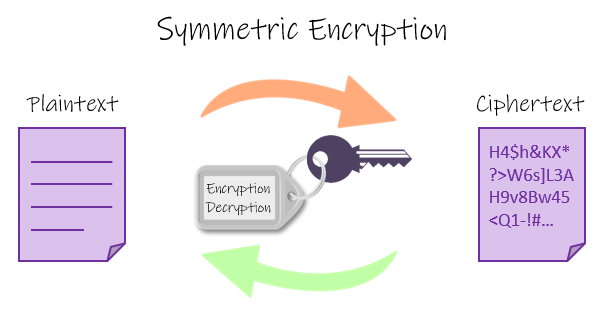
\includegraphics[scale=0.3]{beamer/images/symmetric-encryption.png}
                \end{figure}
                }
                Key: a $n$-bit string
            \end{block}
        }
        \end{column}
        \begin{column}{0.45\textwidth}
            \uncover<3->{
            \begin{block}{Asymmetric encryption}
                \visible<3->{
                \begin{figure}
                    \centering
                    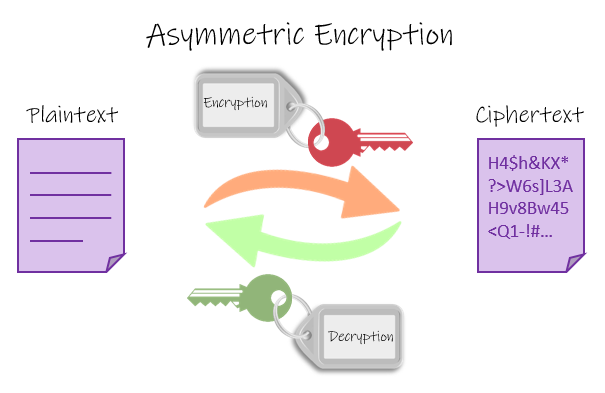
\includegraphics[scale=0.3]{beamer/images/asymmetric-encryption.png}
                \end{figure}
                    }
                Key: the product of two prime numbers, \emph{i.e.} $n=p\cdot q$
            \end{block}
            }
        \end{column}
    \end{columns}
\end{frame}


\begin{frame}{Cryptanalytic attacks}
    What are the best attacks on modern cryptosystems?
    \begin{block}{On Classical Computers}
        \begin{itemize}
            \uncover<1->{\item Symmetric: exhaustive search, $\mathcal{O}(2^n)$}
            \uncover<2->{\item Asymmetric: General Number Field Sieve, $\approx \mathcal{O}(2^{n-\epsilon})$}
        \end{itemize}
    \end{block}

    \begin{block}{On Quantum Computers}
        \begin{itemize}
            \uncover<3->{\item Symmetric: Grover's algorithm, $\mathcal{O}(\sqrt{2^n})$}
            \uncover<4->{\item Asymmetric: Shor's algorithm, $\approx \mathcal{O}((\log{n})^2)$}
        \end{itemize}
    \end{block}
    \uncover<5->{Shor's algorithm can break asymmetric cryptosystems in polynomial time!}
\end{frame}

\begin{frame}{The Computational Complexity Zoo}
    \vspace{15pt}
    \begin{figure}
        \centering
        \only<1>{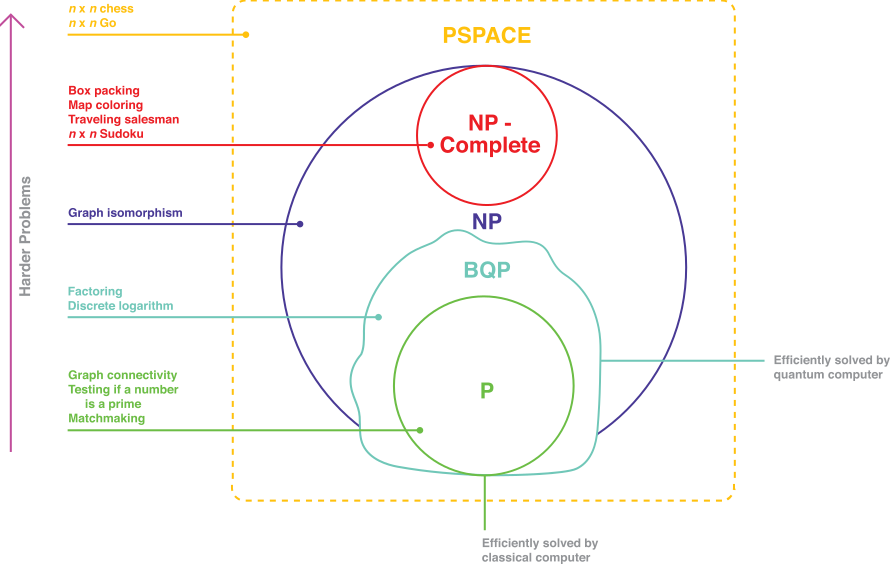
\includegraphics[scale=0.35]{beamer/images/bqp1.png}}
        \only<2>{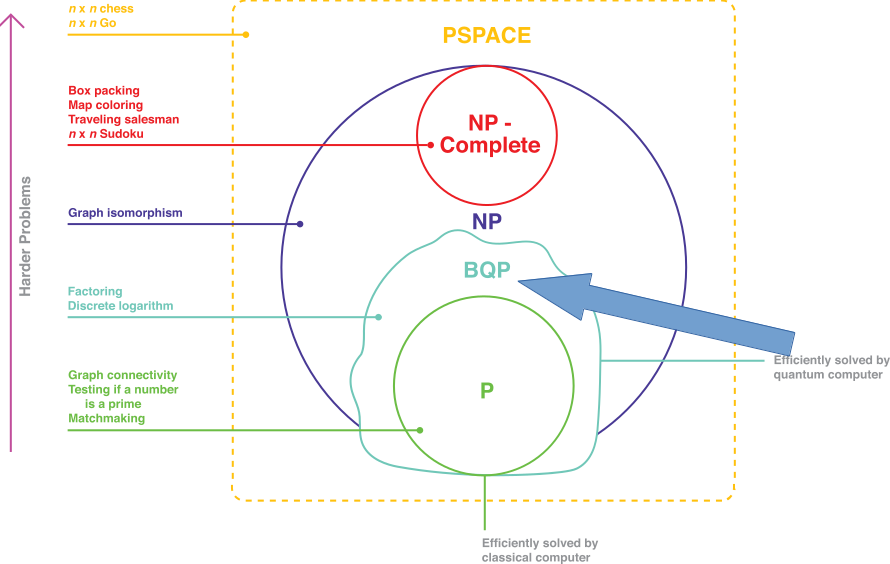
\includegraphics[scale=0.35]{beamer/images/bqp2.png}}
        \only<3>{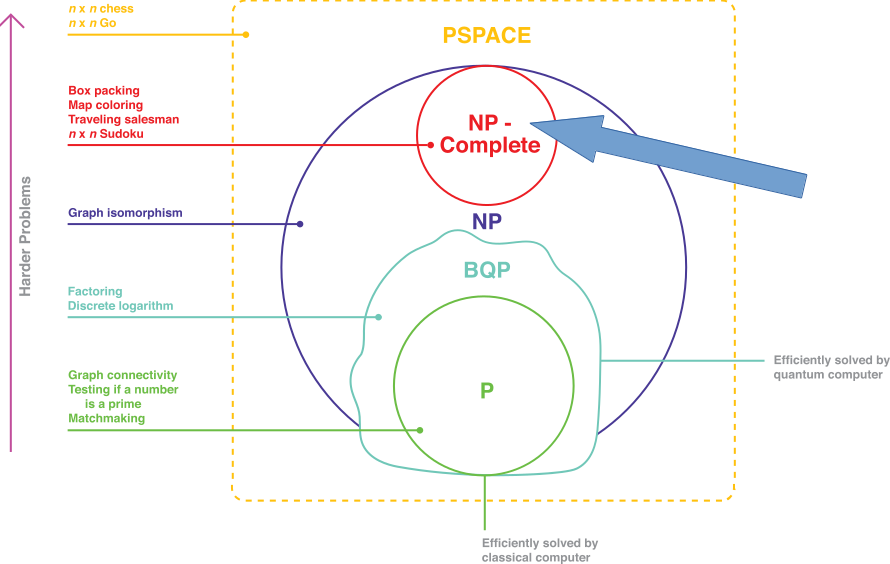
\includegraphics[scale=0.35]{beamer/images/bqp3.png}}
    \end{figure}
\end{frame}

\begin{frame}{NIST Post-Quantum Cryptography Standardization}
    \begin{block}{Timeline}
        \begin{itemize}
            \uncover<1->{\item 26/02/16: Announcement of NIST's call for submissions}
            \uncover<2->{\item 21/12/17: Announcement of the first round candidates (69)
            \item 30/01/19: Announcement of the second round candidates (26)
            \item 22/07/20: Announcement of the third round candidates\\ (7 finalists, 8 alternatives)}
            \uncover<3->{\item 05/07/22: Announcement of the fourth round candidates (4)
            \item 2022-2024: Publication of the standard drafts}
        \end{itemize}
    \end{block}
\end{frame}

\begin{frame}{Standardization candidates}
    \begin{block}{Third Round winner}
        \begin{itemize}
            \item CRYSTALS-Kyber: lattice-based
        \end{itemize}
    \end{block}
    \uncover<2->{
    NIST decided to standardize at least another PQC scheme, in case lattice-based crypto fails
    }
    \uncover<3->{
    \begin{block}{Fourth Round candidates}
        \begin{itemize}
            \item \st{\textbf{S}upersingular \textbf{I}sogeny \textbf{K}ey \textbf{E}ncapsulation}
            \item \textbf{B}it Fl\textbf{i}pping \textbf{K}ey \textbf{E}ncapsulation~\cite{BIKE}
            \item \textbf{H}amming \textbf{Q}uasi-\textbf{C}yclic~\cite{melchor2018hamming}
            \item Classic McEliece~\cite{ClassicMcEliece}
        \end{itemize}
    \end{block}  
    BIKE, Classic McEliece and HQC are all code-based cryptosystems.
    }
\end{frame}

\subsection{Side channel attacks}
\begin{frame}{}
    \subsectionpage
\end{frame}

\begin{frame}{Side channel attacks}
    \begin{block}{}
        Devices running cryptosystems may expose secrets through \emph{side channels}
        Observable aspects of the system from which information can be extracted
    \end{block}
    \begin{figure}
        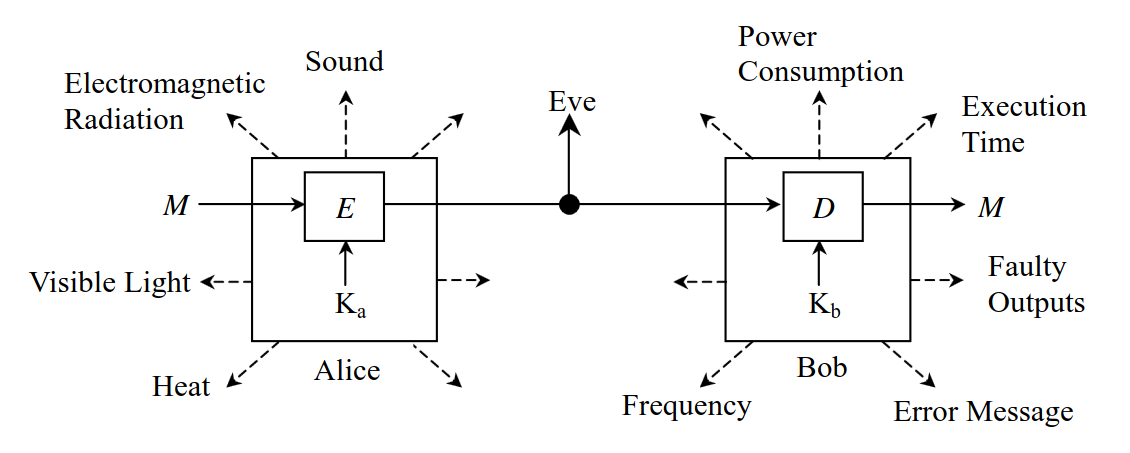
\includegraphics[width=0.8\textwidth]{beamer/images/sca.png}
    \end{figure}
\end{frame}

\begin{frame}{Timing attacks}
    \begin{block}{}
        Execution time may vary based on the inputs
        \begin{itemize}
            \uncover<2->{\item Loops iterating over the input}
            \uncover<3->{\item Branches based on the input}
        \end{itemize}
    \end{block}
    \uncover<4->{
    \begin{block}{Countermeasures}
        Don't use sensitive inputs in branching instructions
        \begin{itemize}
            \item Use constant time algorithms
        \end{itemize}
    \end{block}
    }
\end{frame}

\begin{frame}{Power attacks}
    \begin{block}{}
        Different operations require different amounts of power\\
        Applies to both power and EM attacks
    \end{block}
    \begin{figure}
        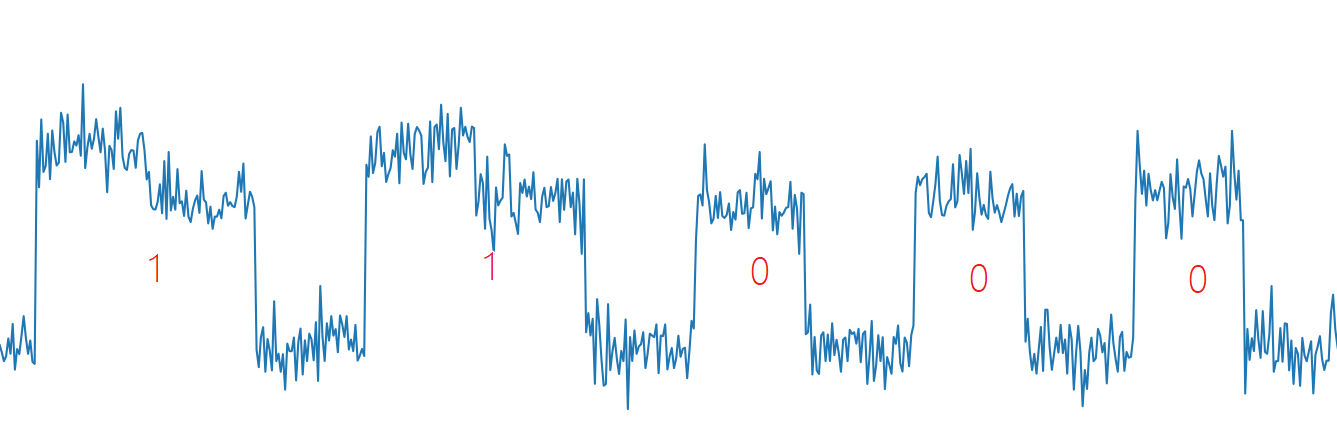
\includegraphics[width=0.6\textwidth]{figures/rsa_squaremult.png}
    \end{figure}
    \uncover<2->{
    \begin{block}{Countermeasures}
        Mask sensitive data with random values
        \begin{itemize}
            \item Makes the power consumption fluctuate randomly
        \end{itemize}
    \end{block}
    }
\end{frame}


\subsection{FFT Butterflies}
\begin{frame}{}
    \subsectionpage
\end{frame}
\begin{frame}{LCH FFT - example}
    Consider a polynomial $f$ in novelpoly basis of degree greater or equal than $\deg (s_k(x)) = 2^k$ and split it in half: 
    \begin{equation*}
        f(x) = p_0(x) + s_k(x)p_1(x)
    \end{equation*}
    \uncover<2->{
    Evaluate $p_0(x)$ and $p_1(x)$ at $\mathbf{W}_{k-1} = \{\alpha \mid \alpha \in \mathbf{W}_{k-1}\}$:
    \begin{equation*}
        p_0(\alpha) + s_k(\alpha)p_1(\alpha)
    \end{equation*}
    }
    \uncover<3->{
    Evaluate $p_0(x)$ and $p_1(x)$ at $(\mathbf{W}_k \setminus \mathbf{W}_{k-1}) = \{\alpha + v_k \mid \alpha \in \mathbf{W}_{k-1}\}$
    \begin{equation*}
        p_0(\alpha+v_k) + s_k(\alpha+v_k)p_1(\alpha+v_k)
    \end{equation*}
    }
    \uncover<4->{
    $p_0(x)$ and $p_1(x)$ are combinations of vanishing polynomials $s_i(x)$ with $i < k$:
    \begin{equation*}
       \sum s_i(\alpha + v_k) = \sum s_i(\alpha) + s_i(v_k) = \sum s_i(\alpha) + 0 = \sum s_i(\alpha)
    \end{equation*}
    }
\end{frame}

\begin{frame}{LCH FFT - example}
    From this consideration, we can observe that:
    \uncover<2->{
    \begin{equation*}
        p_0(\alpha+v_k) = p_0(\alpha), \qquad p_1(\alpha+v_k) = p_1(\alpha)
    \end{equation*}
    }
    \uncover<3->{
    Hence we can rewrite the evaluation at $(\mathbf{W}_k \setminus \mathbf{W}_{k-1})$ as:
    \begin{equation*}
        p_0(\alpha+v_k) + s_k(\alpha+v_k)p_1(\alpha+v_k) = p_0(\alpha) + s_k(\alpha)p_1(\alpha) + s_k(v_k)p_1(\alpha)
    \end{equation*}
    and thus reuse the first evaluation to get the second one.
    }
    \uncover<4->{
    \begin{figure}[H]
    \begin{center}
        \begin{tikzpicture}
            \node (p0) at (0,3) {$p_0(X)$};
            \node (p1) at (0,0) {$p_1(X)$};
            \node (h0) at (10,3) {$h_0(X)$};
            \node (h1) at (10,0) {$h_1(X)$};
            \node (mul) at (3, 0) {$\bullet$};
            \node (add1) at (5, 3) {$\oplus$};
            \node (add2) at (7, 0) {$\oplus$};
            \node (sk) at (3.3, 1.5) {$s_k(\alpha)$};
            % arrow from p3 to p4
            \draw[->] (p0) to (add1);
            \draw[->] (p1) to (mul);
            \draw[->] (mul) to (add1);
            \draw[->] (mul) to (add2);
            \draw[->] (add1) to (add2);
            \draw[->] (add1) to (h0);
            \draw[->] (add2) to (h1);
        \end{tikzpicture}
    \end{center}
    \caption{Butterfly unit}
    \label{fig:butterfly} 
\end{figure}
    }
\end{frame}

\subsection{Fujisaki-Okamoto transformation}
\begin{frame}{}
    \subsectionpage
\end{frame}

\begin{frame}{Key Encapsulation Mechanism}
    By applying the Fujisaki-Okamoto transformation it is possible to build a IND-CCA2 KEM.
    Let $\mathcal{G, H, K}$ be hash functions and $\mathcal{E}$ an instance of \textsf{HQC.PKE}
    \begin{block}{}
        \begin{itemize}
            \item \textbf{Setup}: generate the parameters $\lambda$ as in \textsf{HQC.PKE}, except that k will be the length of the key to be exchanged
            \item \textbf{KeyGen}: as in \textsf{HQC.PKE}
        \end{itemize}
    \end{block}
\end{frame}

\begin{frame}{Key Encapsulation Mechanism}
    Let $\mathcal{G, H, K}$ be hash functions and $\mathcal{E}$ an instance of \textsf{HQC.PKE}
    \begin{block}{Encapsulation}
        \begin{itemize}
            \item Generate the seed $\mathbf{m} \xleftarrow{\$} \mathds{F}_2^k$ and the randomness $\theta \leftarrow \mathcal{G}(\mathbf{m})$
            \item Generate the ciphertext $\mathbf{c} \leftarrow (\mathbf{u, v}) = \mathcal{E}.\textsf{Encrypt}(\textsf{pk}, \mathbf{m}, \theta)$
            \item Derive the symmetric key $K = \mathcal{K}(\mathbf{m, c})$
            \item Calculate $\mathbf{d} \leftarrow \mathcal{H}(\mathbf{m})$
            \item Send the pair $(\mathbf{c, d})$
        \end{itemize}
    \end{block}
\end{frame}

\begin{frame}{Key Encapsulation Mechanism}
    Let $\mathcal{G, H, K}$ be hash functions and $\mathcal{E}$ an instance of \textsf{HQC.PKE}
    \begin{block}{Decapsulation}
        \begin{itemize}
            \item Decrypt $\mathbf{m}^{'} \leftarrow \mathcal{E}.\textsf{Decrypt}(\textsf{sk}, \mathbf{c})$
            \item Compute $\theta^{'} \leftarrow \mathcal{G}(\mathbf{m}^{'})$ and $\mathbf{c}^{'} \leftarrow \mathcal{E}.\textsf{Encrypt}(\textsf{pk}, \mathbf{m}^{'}, \theta^{'})$
            \item Check that $\mathbf{c = c^{'}}$ and $\mathbf{d} = \mathcal{H}(\mathbf{m}^{'})$
            \item Derive the shared key $K \leftarrow \mathcal{K}(\mathbf{m, c})$
        \end{itemize}
    \end{block}
\end{frame}

\subsection{FAFFT Implementation}
\begin{frame}{}
    \subsectionpage
\end{frame}

\begin{frame}{Basis conversion}
    Recursively split the polynomial into halves by dividing by $s_i(x)$\\
    \uncover<2->{
    No actual division required, just XORs:
    \begin{figure}[H]
        \begin{center}
            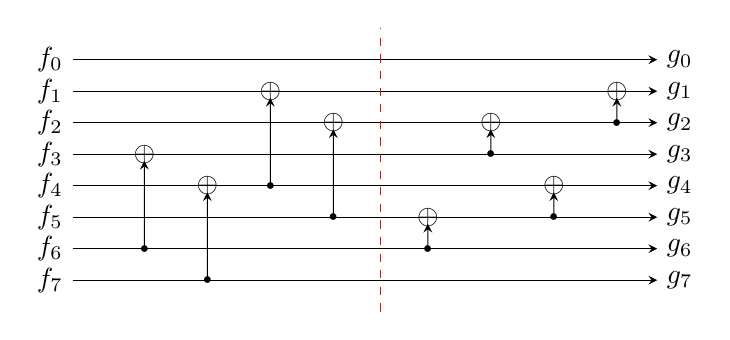
\begin{tikzpicture}[scale=0.4]
                \node (f0) at (0,7) {$f_0$};
                \node (f1) at (0,6) {$f_1$};
                \node (f2) at (0,5) {$f_2$};
                \node (f3) at (0,4) {$f_3$};
                \node (f4) at (0,3) {$f_4$};
                \node (f5) at (0,2) {$f_5$};
                \node (f6) at (0,1) {$f_6$};
                \node (f7) at (0,0) {$f_7$};
                \node (g0) at (20,7) {$g_0$};
                \node (g1) at (20,6) {$g_1$};
                \node (g2) at (20,5) {$g_2$};
                \node (g3) at (20,4) {$g_3$};
                \node (g4) at (20,3) {$g_4$};
                \node (g5) at (20,2) {$g_5$};
                \node (g6) at (20,1) {$g_6$};
                \node (g7) at (20,0) {$g_7$};
    
                \node (m1) at (3, 1)  {\tiny$\bullet$};
                \node (m2) at (5, 0)  {\tiny$\bullet$};
                \node (m3) at (7, 3)  {\tiny$\bullet$};
                \node (m4) at (9, 2)  {\tiny$\bullet$};
                \node (m5) at (12, 1) {\tiny$\bullet$};
                \node (m6) at (14, 4) {\tiny$\bullet$};
                \node (m7) at (16, 2) {\tiny$\bullet$};
                \node (m8) at (18, 5) {\tiny$\bullet$};
    
                \node (a1) at (3, 4)  {$\oplus$};
                \node (a2) at (5, 3)  {$\oplus$};
                \node (a3) at (7, 6)  {$\oplus$};
                \node (a4) at (9, 5)  {$\oplus$};
                \node (a5) at (12, 2) {$\oplus$};
                \node (a6) at (14, 5) {$\oplus$};
                \node (a7) at (16, 3) {$\oplus$};
                \node (a8) at (18, 6) {$\oplus$};
    
                \draw[-stealth] (f0) -- (g0);
                \draw[-stealth] (f1) -- (g1);
                \draw[-stealth] (f2) -- (g2);
                \draw[-stealth] (f3) -- (g3);
                \draw[-stealth] (f4) -- (g4);
                \draw[-stealth] (f5) -- (g5);
                \draw[-stealth] (f6) -- (g6);
                \draw[-stealth] (f7) -- (g7);
    
                \draw[-stealth, shorten >=-4.5pt] (m1.center) -- (a1);
                \draw[-stealth, shorten >=-4.5pt] (m2.center) -- (a2);
                \draw[-stealth, shorten >=-4.5pt] (m3.center) -- (a3);
                \draw[-stealth, shorten >=-4.5pt] (m4.center) -- (a4);
                \draw[-stealth, shorten >=-4.5pt] (m5.center) -- (a5);
                \draw[-stealth, shorten >=-4.5pt] (m6.center) -- (a6);
                \draw[-stealth, shorten >=-4.5pt] (m7.center) -- (a7);
                \draw[-stealth, shorten >=-4.5pt] (m8.center) -- (a8);
    
                \draw[dashed, color=red] (10.5, -1) -- (10.5, 8);
    
                
            \end{tikzpicture}
        \end{center}
    \end{figure}
    }
    \uncover<3->{
    Also, skip the (padded) null coefficients
    }
\end{frame}

\begin{frame}{Evaluation with the FFT}
    \begin{block}{Frobenius partition}
        Polynomial degree $2\cdot 17669 \rightarrow n = 65536$\\
        32-bit words $\rightarrow m = 32$\\
        \uncover<2->{
        Optimal Frobenius partition:
        \begin{equation*}
            \mathbf{S} = v_{l+m/2} + \mathbf{W}_l  = v_{27} + \mathbf{W}_{11}
        \end{equation*}
        with $l = \log_2(n/m)$
        }
    \end{block}
    \uncover<3->{
    \begin{block}{Encoding}
        The first $\log_2(m)$ layers of the FFT use multipliers depending only on $m$
        \begin{itemize}
            \uncover<4->{\item Encode (truncated FFT) the first $\log_2(m)$ recursion layers}
            \uncover<5->{\item \emph{Classic} butterflies for the remaining layers}
        \end{itemize}
    \end{block}
    }
\end{frame}

\begin{frame}{Encoding}
    \begin{block}{}
        The first $l_m = \log_2(m)$ layers of the FFT convert elements from
        $\mathds{F}_2^n$ to $\mathds{F}_{2^m}^{n^\prime}$.\\
        \uncover<2->{
        The twiggle factors can be rewritten as
        \begin{equation*}
            \begin{aligned}
                s_{l+1}(v_{l+m/2}), &\cdots, s_{l+l_m}(v_{l+m/2}) \\
                v_{m/2-1}, &\cdots, v_{m/2-l_m}
            \end{aligned}
        \end{equation*}
        }
        \uncover<3->{
        so the encoding can be implemented as a linear map:
        \begin{equation*}
            g_i = \sum_{j=0}^{m-1} f_{j\cdot n^\prime +i}\cdot r_j = \begin{bmatrix} f_{0\cdot n^\prime} & f_{1\cdot n^\prime} & \cdots &f_{(m-1)\cdot n^\prime}\end{bmatrix} \cdot \begin{bmatrix}

                r_0 \\
                r_1 \\
                \vdots \\
                r_{m-1}
            \end{bmatrix}
        \end{equation*}
        }
    \end{block}
\end{frame}

\begin{frame}{Multiplications}
    \begin{block}{Butterfly twiggle factors}
        Multiplication step: $\beta\cdot p_1(s_1(\beta))$, $\beta = (v+w) \in v_{l+m/2-i} + \mathbf{W}_{l-i}$\\
        \begin{itemize}
            \uncover<2->{\item Precompute and store all the $\beta$ values}
            \uncover<3->{\item Notice that $\gamma\cdot\beta = \gamma\cdot(v+w) = \gamma\cdot v + \gamma\cdot w$}
            \uncover<4->{
            \begin{itemize}
                \item $\gamma\cdot v$ can be computed with a binary circuit ($v$ are fixed)
                \item $\gamma\cdot w$ can be computed in a subfield to reduce the number of bits
            \end{itemize}
            }
        \end{itemize}
    \end{block}
    \uncover<5->{
    \begin{block}{Pointwise multiplications}
    The resulting evaluation points are, by construction, in $\mathds{F}_{2^{32}}$.\\
    Apply Karatsuba (only once) to operate in $\mathds{F}_{2^{16}}$ and have the results
    fit in the 32-bit CPU registers.
    \end{block}
    }
\end{frame}